\section{研究動機}

這是大致的規劃



\begin{figure}
    \centering
    % [width=0.8\textwidth,natwidth=610,natheight=642]
    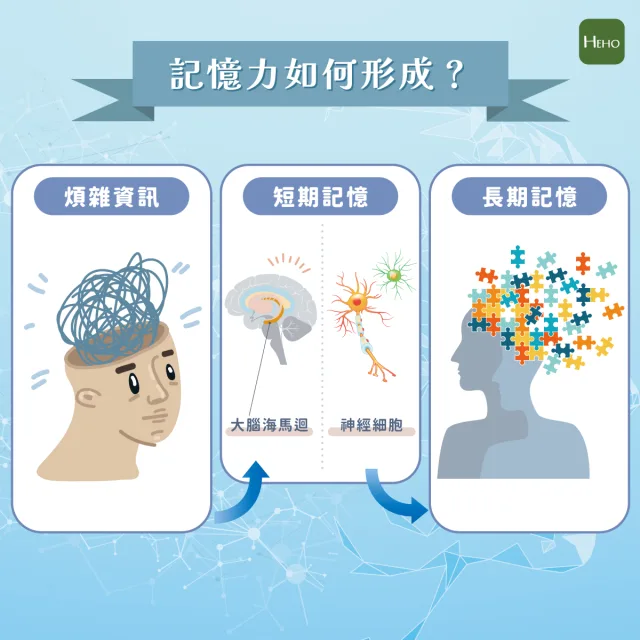
\includegraphics[width=0.5\linewidth,natwidth=600,natheight=600]{figures/3ac2dbd72f1431bb1ffde8fc28724640.webp}
    \caption{Enter Caption2}
    \label{fig:enter-label2}
\end{figure}

\begin{figure}
    \centering
    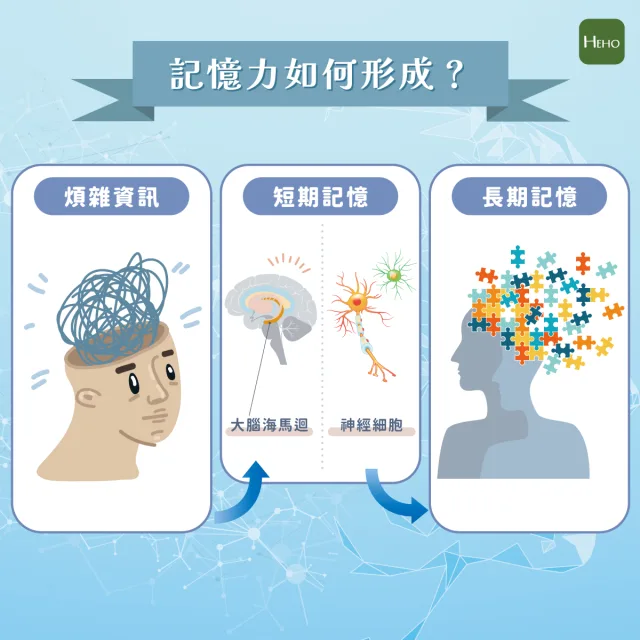
\includegraphics[width=0.5\linewidth]{figures/3ac2dbd72f1431bb1ffde8fc28724640.png}
    \caption{Enter Captddion}
    \label{fig:enter-labddel}
\end{figure}

\begin{figure}
    \centering
    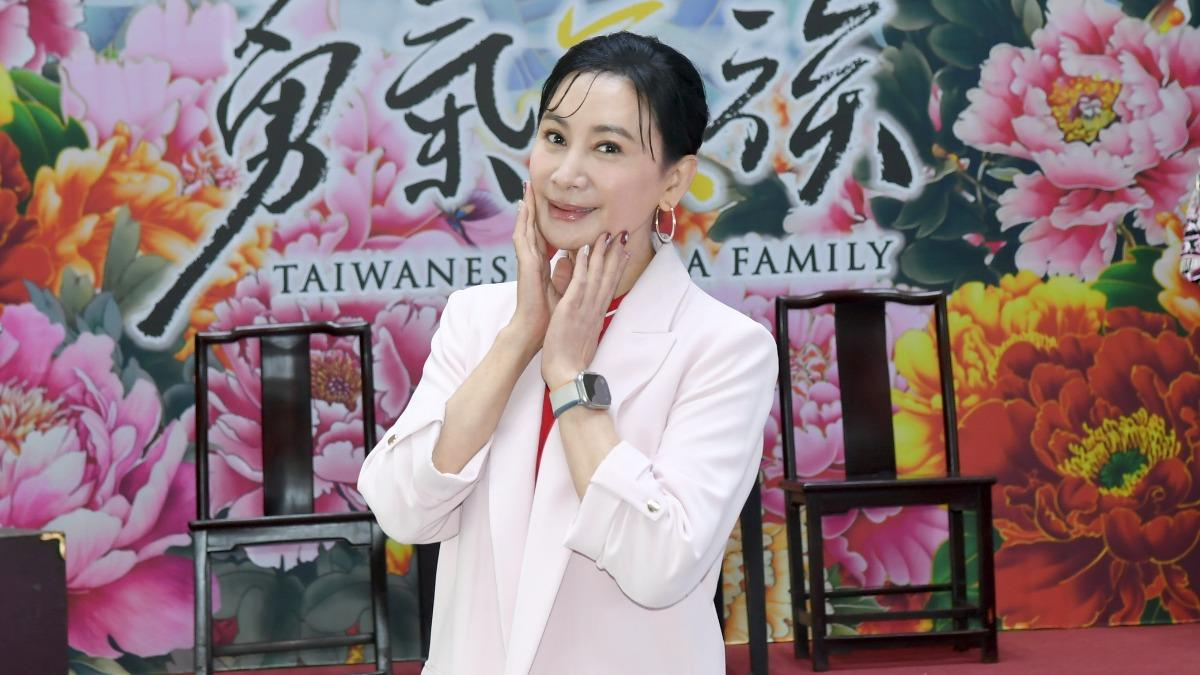
\includegraphics[width=0.5\linewidth]{figures/20240511141026-0fed3f0a.jpg}
    \caption{Enter Caption}
    \label{fig:enter-label}
\end{figure}



% https://stackoverflow.com/questions/56826748/keeping-figure-just-after-text-in-latex
\begin{figure}[hbt!]
    \centering
    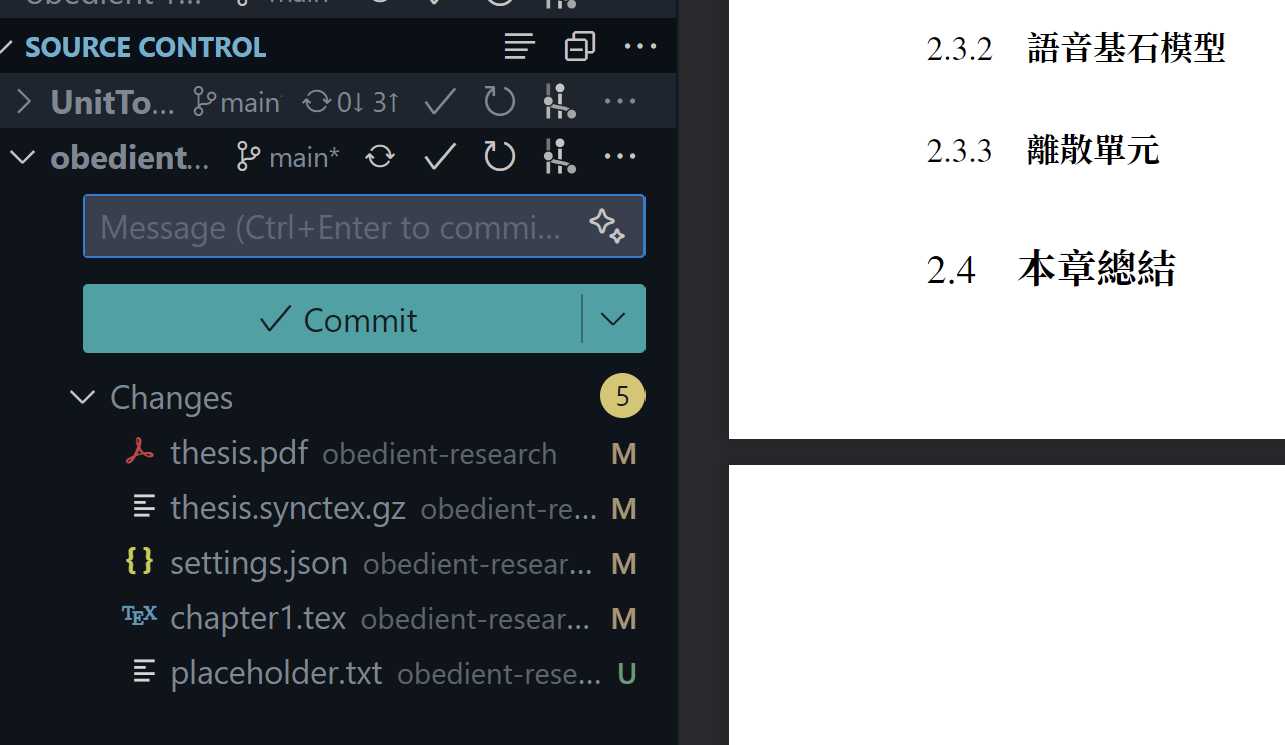
\includegraphics{figures/figfake1.png}
    \caption{整個的系統 system}
    \label{fig:mysts}
\end{figure}

根據圖 \ref{fig:mysts} 中顯示


% ================================================== %

\section{章節安排}
希望可以開始
本論文之章節安排如下:

\begin{itemize}
  \itemsep -2pt %reduce space between items
  \item  第二章:介紹本論文相關背景知識。
  \item  第三章:介紹A。
  \item  第四章:介紹B。
  \item  第五章:介紹C。
  \item  第六章:本論文之結論與未來研究方向。
\end{itemize}


% ~~~~~~~~~~~~~~~~~~~~~~~~~~~~~~~~~~~~~~~~~~~~~~~~~~~~
% Ch1

%%%%% % !TeX root = ../../thesis.tex
%%%%% 
%%%%% \chapter{導論}  %% 確定!不是緒論!
%%%%% 
%%%%% \section{研究動機}
%%%%% 
%%%%% 
%%%%% \section{研究方向}  %% 原 {研究主題}
%%%%% 
%%%%% 
%%%%% \section{主要貢獻}  %% 這邊被加上去的
%%%%% 
%%%%% \section{章節安排}

% ~~~~~~~~~~~~~~~~~~~~~~~~~~~~~~~~~~~~~~~~~~~~~~~~~~~~
% Ch2

%%%%%% \chapter{背景知識}
%%%%%%     \section{深層類神經網路(deep neural network)}
%%%%%%         % \subsection{簡介} % not necessary?
%%%%%%         \subsection{卷積式(convolutional)類神經網路}
%%%%%%         \subsection{遞迴式(recurrent)類神經網路}
%%%%%%         \subsection{序列至序列(sequence-to-sequence)模型}
%%%%%%         \subsection{專注(attention)機制}    
%%%%%%         \subsection{轉換器(Transformer)}
%%%%%%     \section{表徵(representation)學習}
%%%%%%         \subsection{文字的語意表徵}
%%%%%%         \subsection{語音特徵與表徵}
%%%%%%     \section{語音基石模型與自監督式學習}
%%%%%%         \subsection{自監督式學習}
%%%%%%         \subsection{語音基石模型}
%%%%%%         \subsection{離散單元}
%%%%%% \section{本章總結}
  

% ~~~~~~~~~~~~~~~~~~~~~~~~~~~~~~~~~~~~~~~~~~~~~~~~~~~~
% Ch1

%%%%% % !TeX root = ../../thesis.tex
%%%%% 
%%%%% \chapter{導論}  %% 確定!不是緒論!
%%%%% 
%%%%% \section{研究動機}
%%%%% 
%%%%% 
%%%%% \section{研究方向}  %% 原 {研究主題}
%%%%% 
%%%%% 
%%%%% \section{主要貢獻}  %% 這邊被加上去的
%%%%% 
%%%%% \section{章節安排}

